\section{Базис векторного пространства. Системы координат.}

\subsection{Пространства}

\begin{definition}
	Множество назовем $\textit{замкнутым}$ относительно операции, если результат применения этой операции принадлежит этому множеству.
\end{definition}

\begin{definition}
	Непустое множество, замкнутое относительно линейных операций (сложение и умножение на число), назовем $\textit{векторным пространством}$.
\end{definition}

Если одно векторное пространство является подмножеством другого, будем называть его $\textit{подпространством}$.

Само множество является своим подмножеством $\longrightarrow$ пространство является своим подпространством.


\subsection{Базис в векторном пространстве}

\begin{definition}
	$\textit{Базис в векторном пространстве}$ $-$ упорядоченный линейно независимый набор векторов, такой, что любой вектор пространства раскладывается по этим векторам.
\end{definition}

В нулевом пространстве базиса нет.

В одномерном пространстве базис $-$ любой ненулевой вектор.

В двумерном пространстве базис $-$ упорядоченная пара неколлинеарных векторов.

В трехмерном пространстве базис $-$ упорядоченная тройка некомпланарных векторов.\\

Любой вектор раскладывается по векторам базиса, и это разложение единственно.\\

Пусть существует базис ($\overline{e_1}, \overline{e_2}, \overline{e_3}$), такой что любой вектор в этом базисе $\overline{a} = x_1\overline{e_1} + x_2\overline{e_2} + x_3\overline{e_3}$. Тогда коэффициенты разложения $x_1$, $x_2$, $x_3$ определяются единственным образом и называются $\textit{координатами}$.\\

Пусть в этом же базисе существуют вектора $\overline{a}(a_1, a_2, a_3), \overline{b}(b_1, b_2, b_3), \overline{c}(c_1, c_2, c_3)$. Узнаем, является ли этот набор линейно зависимым. Для этого необходимо узнать, существует ли их нетривиальная комбинация:

\begin{center}
	$\alpha\overline{a} + \beta\overline{b} + \gamma\overline{c} = \overline{0}\tab\longleftrightarrow$\\
	
	$\alpha
	\begin{pmatrix*}
		a_1\\
		a_2\\
		a_3\\
	\end{pmatrix*} + \beta
	\begin{pmatrix*}
		b_1\\
		b_2\\
		b_3\\
	\end{pmatrix*} + \gamma
	\begin{pmatrix*}
		c_1\\
		c_2\\
		c_3\\
	\end{pmatrix*} = 
	\begin{pmatrix*}
		0\\
		0\\
		0\\
	\end{pmatrix*}$
\end{center} $\longrightarrow$ по теореме Крамера система имеет единственное решение, отличное от тривиальной комбинации, при
\begin{center}
	det = 
	$\begin{vmatrix}
		a_1 & b_1 & c_1\\
		a_2 & b_2 & c_2\\
		a_3 & b_3 & c_3\\
	\end{vmatrix} \longrightarrow$ если det = 0, система линейно зависима, иначе $-$ линейно независима.
	
\end{center}

Аналогично для плоскости.

\subsection{Декартова и некоторые другие системы координат}

\begin{wrapfigure}{l}{0.4\textwidth}
	\includegraphics[width=0.5\linewidth]{images/дск.jpeg}
\end{wrapfigure}

\begin{definition}
	\textit{Декартова система координат} $-$ совокупность точки и базиса.
\end{definition}

\tab\\ \tab\\
O $-$ начало координат\\
$\overline{e_1}, \overline{e_2}, \overline{e_3}$ $-$ базис\\
$\overline{OM}$ = $x_1\overline{e_1} + x_2\overline{e_2} + x_3\overline{e_3}$ $\longrightarrow$ $x_1, x_2, x_3$ $-$ координаты.

\tab\\ \tab\\ \tab\\ \tab\\ \tab\\

\textbf{Медианный вектор}\\

\begin{wrapfigure}{r}{0.4\textwidth}
	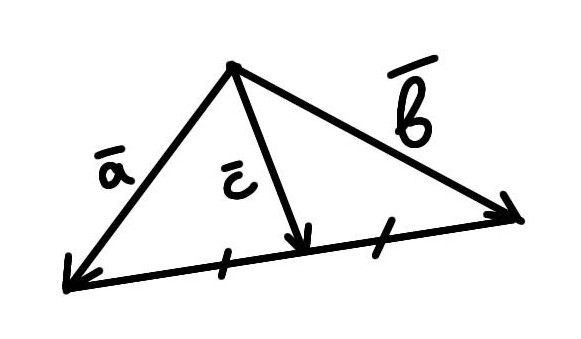
\includegraphics[width=0.8\linewidth]{images/медианныйвектор.jpeg}
\end{wrapfigure}

Пусть $\overline{a}, \overline{b}$ $-$ образующие векторы, $\overline{c}$ $-$ медианный. Тогда $\overline{c}$ = $\frac{\overline{a} + \overline{b}}{2}$.\\

Аналогично можно найти координаты середины отрезка, с концами в координатах ($a_1, a_2, a_3$) и ($b_1, b_2, b_3$), M = ($\frac{a_1 - b_1}{2}, \frac{a_2 - b_2}{2}, \frac{a_3 - b_3}{2}$)

\tab\\ \tab\\

\textbf{Вектор, коллинеарный биссектрисе угла}

\begin{wrapfigure}{l}{0.4\textwidth}
	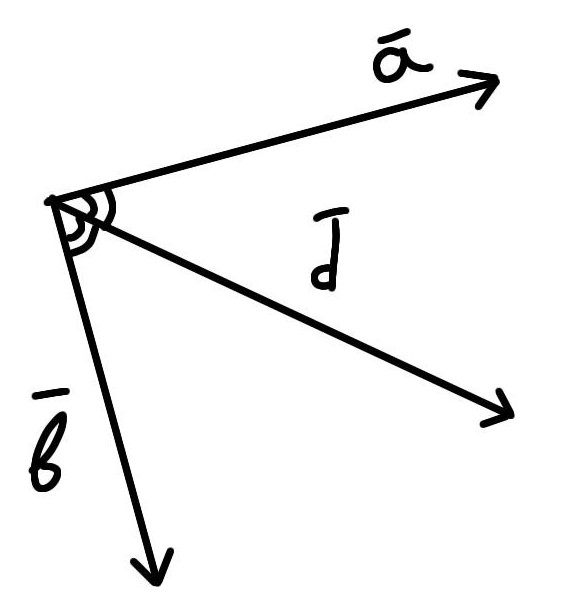
\includegraphics[width=0.6\linewidth]{images/биссектриса.jpeg}
\end{wrapfigure}

\tab\\ \tab\\

Пусть $\overline{d}$ $-$ вектор, коллинеарный биссектрисе угла, построенного на векторах $\overline{a}$ и $\overline{b}$.\\
 
$\overline{d}$ = $\frac{\overline{a}}{|\overline{a}|} + \frac{\overline{b}}{|\overline{b}|}$

\tab\\ \tab\\ \tab\\ \tab\\
\textbf{Вектор, который делит прямую в соотношении m:n}

\begin{wrapfigure}{r}{0.4\textwidth}
	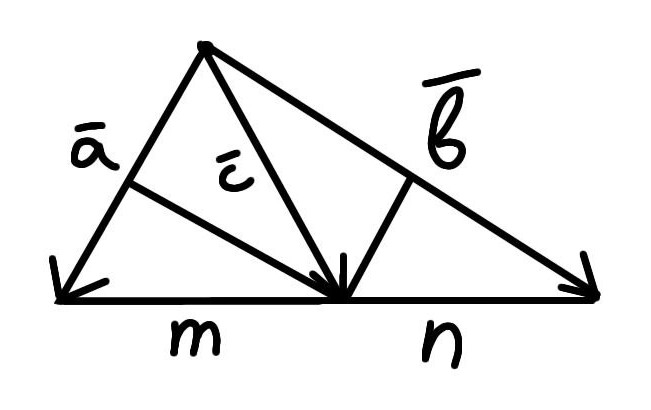
\includegraphics[width=0.6\linewidth]{images/соотношение.jpeg}
\end{wrapfigure}

\tab\\

$\overline{c}$ = $\frac{n}{m + n}\overline{a} + \frac{m}{m + n}\overline{b}$

\tab\\ \tab\\ \tab\\ \tab\\

\begin{definition}
	Если базисные векторы попарно ортогональны, то базис \textit{ортогональный}.
\end{definition}

\begin{definition}
	Если базисные векторы попарно ортогональны, а их длины равны 1, то базис \textit{ортонормированный} (ОНБ).
\end{definition}

\begin{definition}
	Система координат с ОНБ $-$ \textit{декартова прямоугольная система координат}.
\end{definition}

\textbf{Полярная система координат}\\
\begin{wrapfigure}{l}{0.4\textwidth}
	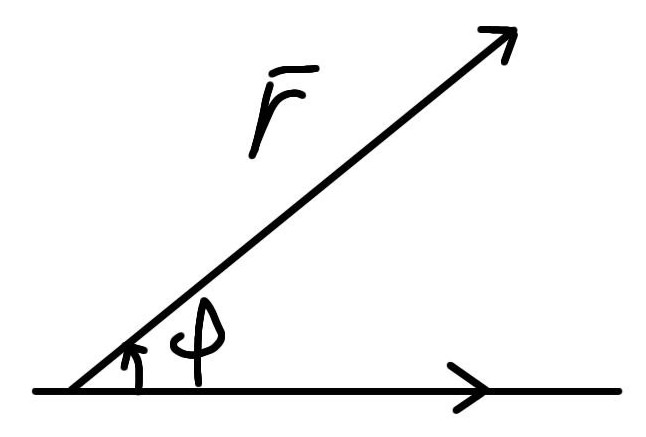
\includegraphics[width=0.6\linewidth]{images/полярнаяск.jpeg}
\end{wrapfigure}

Координаты задаются длиной радиус-вектора $\overline{r}$ и полярным углом $\phi$.\\

$\overline{r}(|\overline{r}|, \phi)$

\tab\\ \tab\\ \tab\\

\textbf{Цилиндрическая система координат}\\
\begin{wrapfigure}{l}{0.4\textwidth}
	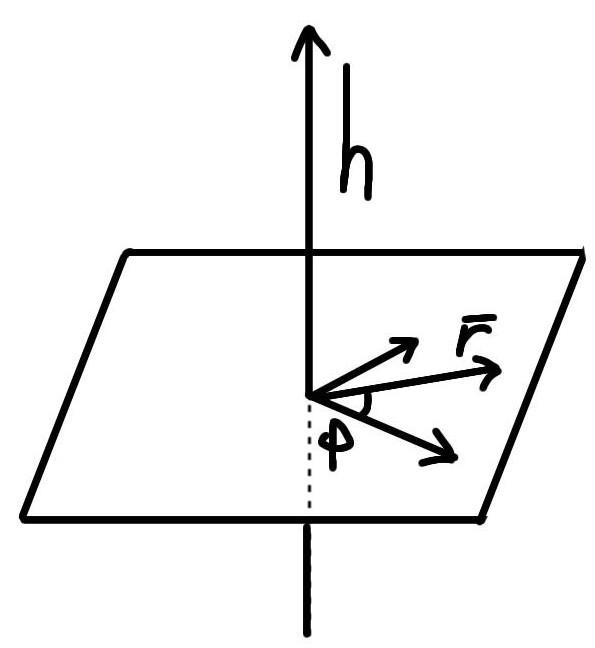
\includegraphics[width=0.6\linewidth]{images/цилиндрическаяск.jpeg}
\end{wrapfigure}

Координаты задаются длиной радиус-вектора $\overline{r}$, полярным углом $\phi$ и смещением относительно оси z.\\

$\overline{r}(|\overline{r}|, \phi, h)$

\tab\\ \tab\\ \tab\\ \tab\\ \tab\\ \tab\\
\textbf{Сферическая система координат}\\
\begin{wrapfigure}{l}{0.4\textwidth}
	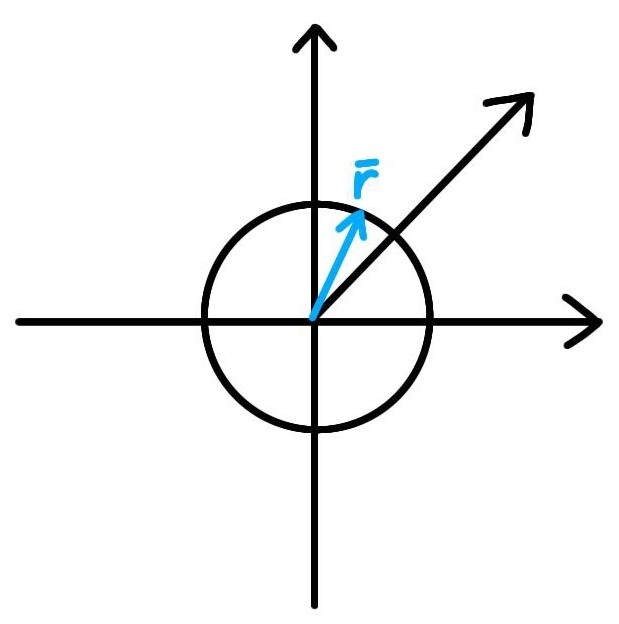
\includegraphics[width=0.5\linewidth]{images/сферическая.jpeg}
\end{wrapfigure}

Координаты задаются длиной радиус-вектора $\overline{r}$, азимутальным углом $\phi\in[0, 2\pi]$ и зенитным углом $\theta\in[-\frac{\pi}{2}, \frac{\pi}{2}]$.\\

$\overline{r}(|\overline{r}|, \theta, \phi)$
\tab\\ \tab\\ \tab\\ \tab\\ \tab\\
\newpage

\subsection{Переход в новую систему координат}

Пусть имеются две системы координат и вектор $\overline{a}$:\\
\tab\\
$\tab$($\overline{e_1}, \overline{e_2}, \overline{e_3})$ $-$ "старая" система координат, $\overline{a}$(x, y, z)\\
$\tab$($\overline{e_1'}, \overline{e_2'}, \overline{e_3'})$ $-$ "новая" система координат, $\overline{a}$(x', y', z')\\

Тогда базисные векторы новой системы координат выражаются следующим образом:\\
\tab\\
$\overline{e_1'}$ = $a_{11}\overline{e_1} + a_{21}\overline{e_2} + a_{31}\overline{e_3}$\\
$\overline{e_2'}$ = $a_{12}\overline{e_1} + a_{22}\overline{e_2} + a_{32}\overline{e_3}$\\
$\overline{e_3'}$ = $a_{13}\overline{e_1} + a_{23}\overline{e_2} + a_{33}\overline{e_3}$\\

В новой системе координат $\overline{a}$ = $x'\overline{e_1'} + y'\overline{e_2'} + z'\overline{e_3'}$ = $x'(a_{11}\overline{e_1} + a_{21}\overline{e_2} + a_{31}\overline{e_3}) + y'(a_{12}\overline{e_1} + a_{22}\overline{e_2} + a_{32}\overline{e_3}) + z'(a_{13}\overline{e_1} + a_{23}\overline{e_2} + a_{33}\overline{e_3})$ = $\overline{e_1}(a_{11}x' + a_{12}y' + a_{13}z') + \overline{e_2}(a_{21}x' + a_{22}y' + a_{23}z') + \overline{e_3}(a_{31}x' + a_{32}y' + a_{33}z')\tab\longrightarrow$\\
\tab\\
x = $a_{11}x' + a_{12}y' + a_{13}z'$\\
y = $a_{21}x' + a_{22}y' + a_{23}z'$\\
z = $a_{31}x' + a_{32}y' + a_{33}z'$\\

\begin{definition}
	\textit{Матрица перехода} от базиса e к базису e' имеет вид\\
	\begin{center}
		S =
		$\begin{pmatrix}
			a_{11} & a_{12} & a_{13}\\
			a_{21} & a_{22} & a_{23}\\
			a_{31} & a_{32} & a_{33}\\
		\end{pmatrix}$
	\end{center} 
\end{definition}

Столбцами S являются координаты новых базисных векторов в старом базисе.\\

\begin{center}
	$\begin{pmatrix*}
		x\\
		y\\
		z\\
	\end{pmatrix*}$ = S
	$\begin{pmatrix*}
		x'\\
		y'\\
		z'\\
	\end{pmatrix*}$, $\tab$ ($\overline{e_1'}, \overline{e_2'}, \overline{e_3'}$) = ($\overline{e_1}, \overline{e_2}, \overline{e_3}$)S, $\tab$ e' = eS
\end{center}

\textbf{Основное свойство матрицы перехода:} по теореме о линейной независимости, det S $\neq$ 0.

Рассмотрим старое начало координат О и новое О'. Тогда вектор, соединяющий их\\

\begin{wrapfigure}{l}{0.4\textwidth}
	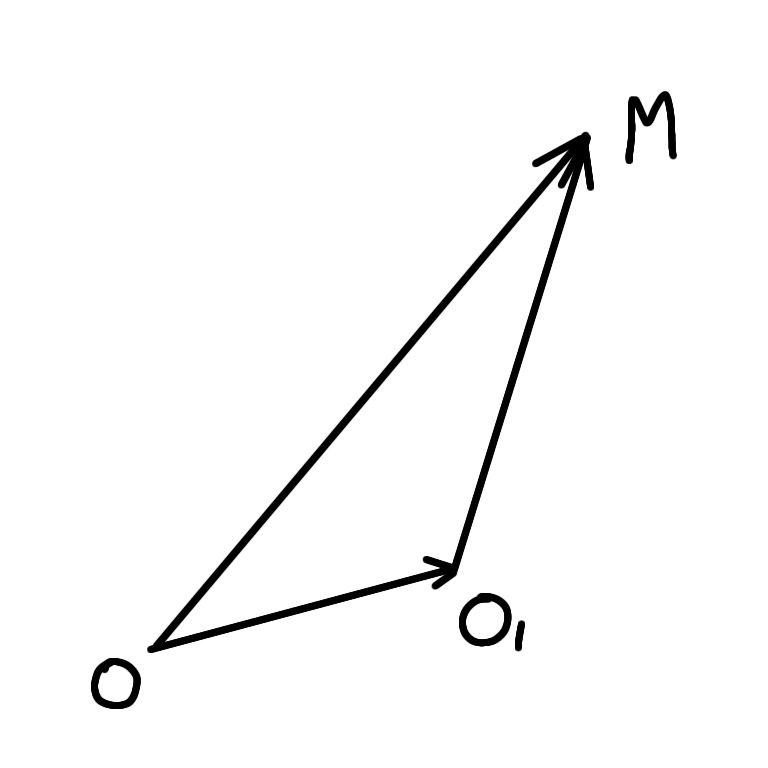
\includegraphics[width=0.6\linewidth]{images/переход1.jpeg}
\end{wrapfigure}

$\overline{OO'}$ = $\beta_1\overline{e_1} + \beta_2\overline{e_2} + \beta_3\overline{e_3}$ \\

Пусть существует произвольная точка М, такая что $\overline{OM}$ = $\overline{OO'} + \overline{O'M}$. Тогда ее координаты\\

x = $a_{11}x' + a_{12}y' + a_{13}z' + \beta_1$\\
y = $a_{21}x' + a_{22}y' + a_{23}z' + \beta_2$\\
z = $a_{31}x' + a_{32}y' + a_{33}z' + \beta_3$\\
